\documentclass[tikz,border=8pt]{standalone}
% Shared look for every TikZ diagram. Load with % Shared look for every TikZ diagram. Load with % Shared look for every TikZ diagram. Load with \input{../../tools/tikz-style.tex}
\usepackage[T1]{fontenc}
\usepackage{lmodern}
\renewcommand{\sfdefault}{lmr}  % diagrams use the same serif as the text
\usetikzlibrary{arrows.meta, positioning, shapes.geometric, calc, fit, backgrounds}
\definecolor{cblue}{HTML}{4C78A8}
\definecolor{corange}{HTML}{F58518}
\definecolor{cgreen}{HTML}{54A24B}
\definecolor{cred}{HTML}{E45756}
\definecolor{cpurple}{HTML}{B279A2}
\definecolor{cgrey}{HTML}{6B6B6B}
\tikzset{
  every picture/.style={font=\sffamily, line width=1.2pt},
  box/.style={draw=#1, fill=#1!12, rounded corners=4pt, align=center, inner sep=7pt, minimum height=1.1cm},
  box/.default=cgrey,
  arrow/.style={-{Stealth[length=3mm]}, draw=cgrey, line width=1.4pt},
  title/.style={font=\sffamily\bfseries\Large},
  note/.style={font=\sffamily\small, text=cgrey, align=center},
}
\AtBeginDocument{\hyphenpenalty=10000 \exhyphenpenalty=10000}

\usepackage[T1]{fontenc}
\usepackage{lmodern}
\renewcommand{\sfdefault}{lmr}  % diagrams use the same serif as the text
\usetikzlibrary{arrows.meta, positioning, shapes.geometric, calc, fit, backgrounds}
\definecolor{cblue}{HTML}{4C78A8}
\definecolor{corange}{HTML}{F58518}
\definecolor{cgreen}{HTML}{54A24B}
\definecolor{cred}{HTML}{E45756}
\definecolor{cpurple}{HTML}{B279A2}
\definecolor{cgrey}{HTML}{6B6B6B}
\tikzset{
  every picture/.style={font=\sffamily, line width=1.2pt},
  box/.style={draw=#1, fill=#1!12, rounded corners=4pt, align=center, inner sep=7pt, minimum height=1.1cm},
  box/.default=cgrey,
  arrow/.style={-{Stealth[length=3mm]}, draw=cgrey, line width=1.4pt},
  title/.style={font=\sffamily\bfseries\Large},
  note/.style={font=\sffamily\small, text=cgrey, align=center},
}
\AtBeginDocument{\hyphenpenalty=10000 \exhyphenpenalty=10000}

\usepackage[T1]{fontenc}
\usepackage{lmodern}
\renewcommand{\sfdefault}{lmr}  % diagrams use the same serif as the text
\usetikzlibrary{arrows.meta, positioning, shapes.geometric, calc, fit, backgrounds}
\definecolor{cblue}{HTML}{4C78A8}
\definecolor{corange}{HTML}{F58518}
\definecolor{cgreen}{HTML}{54A24B}
\definecolor{cred}{HTML}{E45756}
\definecolor{cpurple}{HTML}{B279A2}
\definecolor{cgrey}{HTML}{6B6B6B}
\tikzset{
  every picture/.style={font=\sffamily, line width=1.2pt},
  box/.style={draw=#1, fill=#1!12, rounded corners=4pt, align=center, inner sep=7pt, minimum height=1.1cm},
  box/.default=cgrey,
  arrow/.style={-{Stealth[length=3mm]}, draw=cgrey, line width=1.4pt},
  title/.style={font=\sffamily\bfseries\Large},
  note/.style={font=\sffamily\small, text=cgrey, align=center},
}
\AtBeginDocument{\hyphenpenalty=10000 \exhyphenpenalty=10000}

\begin{document}
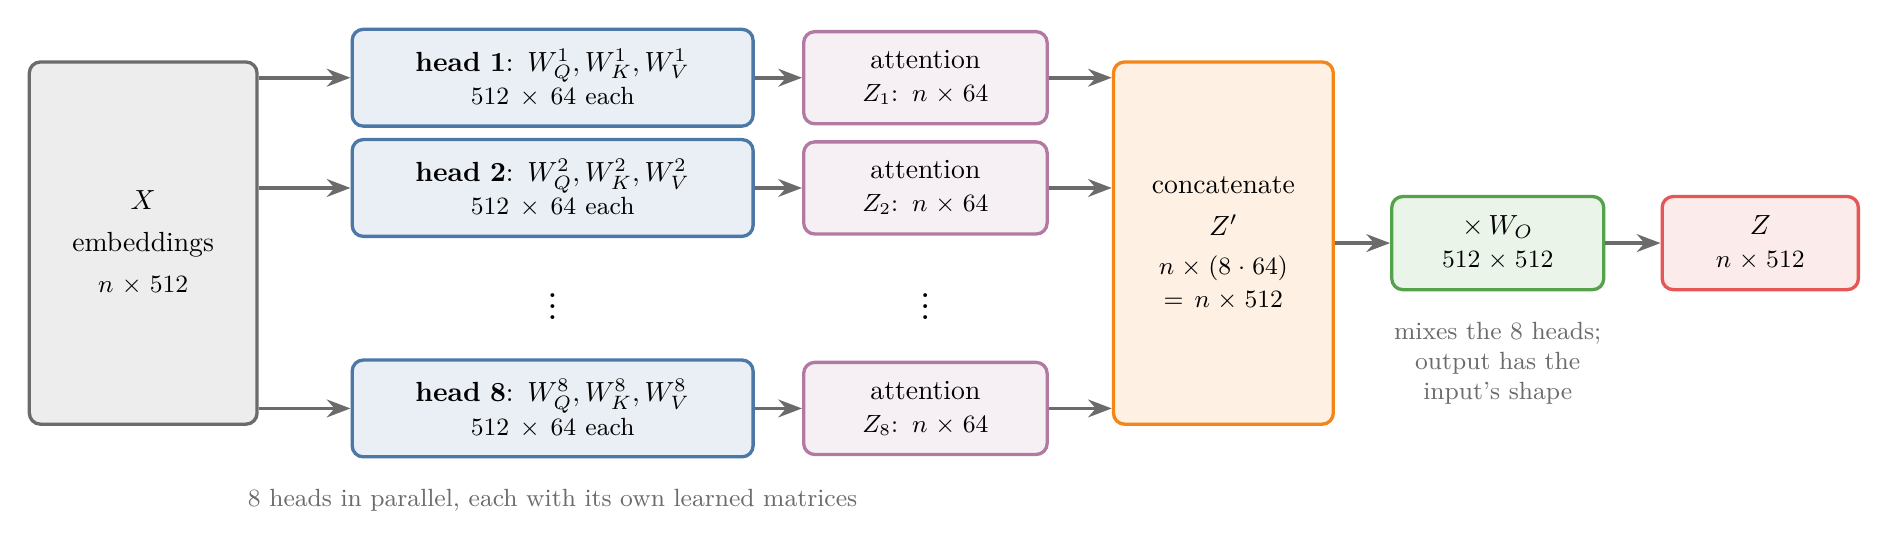
\begin{tikzpicture}[every node/.append style={font=\sffamily}]
  \node[box=cgrey, text width=2.4cm, minimum height=4.6cm] (x) {$X$\\[3pt]embeddings\\[3pt]\small $n \times 512$};
  \foreach \i/\y/\lab in {1/2.1/1, 2/0.7/2, 8/-2.1/8} {
    \node[box=cblue, text width=4.6cm] (h\i) at (5.2,\y) {\textbf{head \lab}: $W_Q^{\lab}, W_K^{\lab}, W_V^{\lab}$\\\small $512 \times 64$ each};
    \node[box=cpurple, text width=2.6cm, right=0.6cm of h\i] (a\i) {attention\\\small $Z_{\lab}$: $n \times 64$};
    \draw[arrow] (x.east |- h\i) -- (h\i);
    \draw[arrow] (h\i) -- (a\i);
  }
  \node[font=\Large] at (5.2,-0.7) {$\vdots$};
  \node[font=\Large] at ($(a2)!0.5!(a8)$) {$\vdots$};
  \node[box=corange, text width=2.3cm, minimum height=4.6cm, right=0.8cm of a2.east |- x] (c) {concatenate\\[3pt]$Z'$\\[3pt]\small $n \times (8 \cdot 64)$\\\small $= n \times 512$};
  \foreach \i in {1,2,8} \draw[arrow] (a\i) -- (a\i -| c.west);
  \node[box=cgreen, text width=2.2cm, right=0.7cm of c] (o) {$\times\, W_O$\\\small $512 \times 512$};
  \node[box=cred, text width=2.0cm, right=0.7cm of o] (z) {$Z$\\\small $n \times 512$};
  \draw[arrow] (c) -- (o);
  \draw[arrow] (o) -- (z);
  \node[note, below=0.25cm of h8] {8 heads in parallel, each with its own learned matrices};
  \node[note, below=0.25cm of o, text width=3.2cm] {mixes the 8 heads;\\output has the input's shape};
\end{tikzpicture}
\end{document}
